\section{Équations maîtres}
\subsection{Équation de Schrödinger et opérateur d'évolution}
\cite{BRE02} L'évolution temporelle d'un système quantique est décrit par la célèbre équation de Schrödinger où on pose ici $\hbar = 1$ :

\begin{equation}
    i\derivative{}{t}\ket{\psi(t)} = H(t)\ket{\psi(t)}
\end{equation}

En définissant un opérateur d'évolution $U(t,t_0)$ qui amène un état du temps $t_0$ au temps $t$, c'est-à-dire que $\ket{\psi(t)} = U(t,t_0)\ket{\psi(t_0)}$, on peut l'injecter dans (1) afin d'avoir 

\begin{equation}
    i \derivative{}{t}U(t,t_0)\ket{\psi(t_0)} = H(t)U(t,t_0)\ket{\psi(t_0)} \implies i \frac{\partial}{\partial t}U(t,t_0) = H(t)U(t,t_0)
\end{equation}

Ici, la dérivée totale devient partielle par la règle de dérivation en chaîne pour les fonctions multivariables. Par ailleurs, il va de soi que $U(t,t) = \mathbb{I}$ pour tout temps $t$, car il n'y a alors, selon notre définition, aucune évolution qui a lieu. Dans ce cas, comme rien ne se passe, il faut que l'opérateur d'évolution soit l'identité. Aussi, on peut décomposer une évolution $U(t, t_0)$ en plusieurs évolutions une à la suite de l'autre de manière à avoir $U(t,t_0) = U(t,t_1)U(t_1,t_0)$ par exemple (il pourrait y en avoir autant qu'on veut).

\subsection{Système fermé et hamiltonien statique}
Pour un système fermé et dont l'hamiltonien est statique (donc indépendant du temps), (1.2) devient

\begin{equation}
    i\frac{\partial}{\partial t}U(t,t_0) = HU(t,t_0) \implies \int_{U(t_0,t_0)}^{U(t,t_0)}\frac{\diff U^{'}}{U'} = -iH \int_{t_0}^{t}dt^{'} \implies U(t,t_0) = e^{-iH(t-t_0)}
\end{equation}

\subsection{Système fermé et hamiltonien dynamique}
Sachant la forme de l'opérateur d'évolution lorsque l'hamiltonien est constant, on peut approximer l'opérateur d'évolution dans le cas où l'hamiltonien est dynamique. En effet, pour une variation infinitésimale de temps $\delta t$, l'hamiltonien change à peine de sa forme de départ et on peut le considérer comme étant constant sur ce petit intervalle. Lorsqu'on dit constant, on veut plutôt dire que l'hamiltonien est évalué à un point fixe à quelque part dans le petit intervalle de temps et ce pour toute la durée de l'opérateur d'évolution. Ainsi, 

\begin{equation*}
    U(t+\delta t, t) \approx e^{-iH(t)\delta t}
\end{equation*}

Ici, on évalue l'hamiltonien à $t$, car de toute manière $\delta t \rightarrow 0$ ce qui en fait un choix pratique. Cependant, on aimerait avoir une forme explicite pour l'opérateur d'évolution sur une plus grande période de temps. On sait qu'on peut découper l'évolution, par exemple, en $N$ sous-intervalles égaux de temps $\epsilon = \frac{t-t_0}{N}$ pour que 

\begin{equation*}
    U(t,t_0) = \prod_{k=1}^{N}U(t_0 + k\epsilon, t_0 + (k-1)\epsilon)
\end{equation*}

Dans la limite où $\epsilon \rightarrow 0$ (donc où $N \rightarrow \infty$), l'approximation plus haut est valide (les sous-intervalles deviennent infiniment petits) et dès lors on peut se dire que

\begin{equation*}
    U(t_0 + k\epsilon, t_0 + (k-1)\epsilon) \approx e^{-i\epsilon H\left(t_0 + (k-1)\epsilon\right)}
\end{equation*}

Alors,

\begin{equation*}
    U(t,t_0) = \lim_{\epsilon \rightarrow 0} \prod_{k=1}^{N}U(t_0 + k\epsilon, t_0 + (k-1)\epsilon) = \lim_{\epsilon \rightarrow 0} \prod_{k=1}^{N} e^{-i\epsilon H(t_0 + (k-1)\epsilon)} = \lim_{\epsilon \rightarrow 0} e^{-i\epsilon H(t_0)}e^{-i\epsilon H(t_0 + \epsilon)} ... e^{-i\epsilon H(t-\epsilon)} 
\end{equation*}

On serait très tenté de combiner les exponentielles en sommant leur argument, mais on travaille avec des matrices et il faut alors faire attention. Effectivement, on peut combiner deux exponentielles contenant une matrice uniquement lorsque ces matrices commutent. Autrement, il faudrait utiliser la formule de Baker-Campbell-Hausdorff qui ne semble pas nous faire progresser avec son infinité de termes. On s'attarde alors aux deux cas possibles.

\subsubsection{Les hamiltoniens commutent}

D'abord, en supposant que tous les $H(t_i)$ dans les exponentielles commutent entre eux, donc que $\left[H(t_i), H(t_j)\right] = 0 \ \forall i,j$, il est possible de combiner toutes les exponentielles de la manière suivante :

\begin{equation}
    U(t,t_0) = \lim_{\epsilon \rightarrow 0} e^{-i \sum_{k=0}^{N-1}H(t_0 + k\epsilon)\epsilon} = e^{-i\int_{t_0}^{t}H(t^{'})dt^{'}}
\end{equation}

On voit clairement que si l'hamiltonien est constant, alors il peut être sorti de l'intégrale redonnant ainsi (1.3).

\subsubsection{Les hamiltoniens ne commutent pas}
Pour ce cas, on utilise une approche itérative. Depuis (1.2) et par une approche similaire à (1.3), on peut écrire 

\begin{equation*}
    \int_{U(t_0,t_0)}^{U(t,t_0)}dU^{'} = -i \int_{t_0}^{t}H(t^{'})U(t^{'}, t_0)dt^{'} \implies U(t,t_0) = \mathbb{I} -i\int_{t_0}^{t}H(t^{'})U(t^{'},t_0)dt^{'}
\end{equation*}

Il ne s'agit pas d'une solution, car on trouve $U(t,t_0)$ des deux côtés de l'équation. Par contre, avec ce fait, on peut remplacer l'équation dans elle-même en prenant soin de changer la notation un peu maladroite pour ce qu'on s'apprête à faire.

\begin{equation*}
    U(t,t_0) = \mathbb{I} -i\int_{t_0}^{t}H(t_1)U(t_1,t_0)dt_1 = \mathbb{I} -i\int_{t_0}^{t}H(t_1)\left(\mathbb{I} - i\int_{t_0}^{t_1}H(t_2)U(t_2,t_0)dt_2\right)dt_1
\end{equation*}
\begin{equation*}
    = \mathbb{I} -i\int_{t_0}^{t}H(t_1)dt_1 - \int_{t_0}^{t}\int_{t_0}^{t_1}H(t_1)H(t_2)U(t_2,t_0)dt_2dt_1
\end{equation*}

On répète le processus à l'infini afin d'obtenir

\begin{equation*}
    U(t,t_0) = \mathbb{I} + \sum_{n=1}^{\infty}(-i)^n \int_{t_0}^{t}\int_{t_0}^{t_1} \ ... \int_{t_0}^{t_{n-1}}H(t_1)H(t_2) ... H(t_n)dt_n ... dt_2 dt_1 
\end{equation*}
\begin{equation}
    = \sum_{n=0}^{\infty}(-i)^n \int_{t_0}^{t}\int_{t_0}^{t_1} \ ... \int_{t_0}^{t_{n-1}}H(t_1)H(t_2) ... H(t_n)dt_n ... dt_2 dt_1  
\end{equation}

ce qu'on appelle une série de Dyson. Par construction, les variables d'intégration respectent $t_1 \geq t_2 \geq ... \geq t_n$ et il est aussi hautement non-trivial de montrer que (1.5) converge. De plus, la notation peut sembler être bizarre pour le terme $n=0$ et $n=1$ avec une borne d'intégration $t_{-1}$ et une intégrale de $t_0$ à $t_0$ respectivement. En tant que tel, à cause de $\int_{t_0}^{t_1} ... \int_{t_0}^{t_{n-1}}$, on comprend implicitement que ça n'a de sens que pour $n\geq2$. Pour le terme $n=0$ et $n=1$, on fait un abus de notation pour les inclure et avoir une équation plus propre. On rappelle ici le terme $n=0$ et $n=1$.

\begin{equation*}
    n=0 : \mathbb{I}, \ n=1 : -i\int_{t_0}^{t}H(t_1)dt_1
\end{equation*}

Il peut être difficile de voir comment (1.5) se réduit à (1.4) ou à (1.3) avec un changement approprié des conditions. On introduit alors l'opérateur de produit chronologique $T$ qui réordonne un produit matriciel de manière à ce que l'argument en temps des matrices dans le produit soit décroissant de la gauche vers la droite. Autrement dit,

\begin{equation}
    T[H(t_1)H(t_2)...H(t_n)] = H(t_{i_1})H(t_{i_2})...H(t_{i_n}) \text{ où } t_{i_1} \geq t_{i_2} \geq ... \geq t_{i_n}
\end{equation}

Évidemment, si tous les hamiltoniens commutent entre eux, alors $T$ ne sert à rien. Pour clarifier l'utilisation de l'opérateur de produit chronologique, on revient à (1.5) en s'attardant à $J_2$ l'intégrale du terme $n=2$ de la somme.

\begin{equation*}
    J_2 = \int_{t_0}^{t}\int_{t_0}^{t_1}H(t_1)H(t_2)dt_2dt_1 
\end{equation*}

Il est important de conserver le même ordre pour la multiplication matricielle, car par hypothèse les hamiltoniens ne commutent pas. Dans cette dernière équation, l'ordre d'intégration fait en sorte que $t_1 \geq t_2$, ce qu'on peut voir en représentant la région d'intégration (qui est la moitié de l'aire d'un carré de côté $t$, voir figure 1 (A)). Ainsi, on peut directement incorporer l'opérateur de produit chronologique dans $J_2$.

\begin{equation*}
    J_2 = \int_{t_0}^{t}\int_{t_0}^{t_1}H(t_1)H(t_2)dt_2dt_1  = \int_{t_0}^{t}\int_{t_0}^{t_1}T\left[H(t_1)H(t_2)\right]dt_2dt_1
\end{equation*}

Sans changer la valeur de $J_2$, on peut changer l'ordre d'intégration de la manière suivante :

\begin{equation*}
    J_2 = \int_{t_0}^{t}\int_{t_2}^{t}H(t_1)H(t_2)dt_1dt_2
\end{equation*}

En représentant cette nouvelle région d'intégration, on voit qu'elle reste la même sauf que maintenant l'intégration se fait "horizontalement" au lieu de "verticalement" (voir figure 1 (B)). On peut ensuite procéder à un changement de variables (qui ne change toujours pas la valeur de $J_2$) où $t_1 \Leftrightarrow t_2$. 

\begin{equation*}
    J_2 = \int_{t_0}^{t}\int_{t_1}^{t}H(t_2)H(t_1)dt_2dt_1
\end{equation*}

La région d'intégration fait alors une réflexion par rapport à l'axe de la droite $t_1=t_2$ et correspond alors à la moitié restante de l'aire du carré de côté $t$ (voir figure 1 (C)). Dans ce cas, $t_2 \geq t_1$ et on écrit 

\begin{equation*}
    J_2 = \int_{t_0}^{t}\int_{t_1}^{t}H(t_2)H(t_1)dt_2dt_1 = \int_{t_0}^{t}\int_{t_1}^{t}T\left[H(t_1)H(t_2)\right]dt_2dt_1
\end{equation*}

Au final, on vient de trouver 2 formes différentes pour $J_2$.

\begin{equation}
    J_2 = \int_{t_0}^{t}\int_{t_0}^{t_1}T\left[H(t_1)H(t_2)\right]dt_2dt_1 = \int_{t_0}^{t}\int_{t_1}^{t}T\left[H(t_1)H(t_2)\right]dt_2dt_1
\end{equation}

On remarque qu'en sommant ensemble chacune des formes, on peut avoir une formule pour $J_2$ où les bornes d'intégration ne dépendent plus des $t_i$. On peut ensuite l'incorporer dans (1.5).

\begin{equation*}
    2J_2 = \int_{t_0}^{t}\int_{t_0}^{t_1}T\left[H(t_1)H(t_2)\right]dt_2dt_1 + \int_{t_0}^{t}\int_{t_1}^{t}T\left[H(t_1)H(t_2)\right]dt_2dt_1 = \int_{t_0}^{t}\int_{t_0}^{t}T\left[H(t_1)H(t_2)\right]dt_2dt_1
\end{equation*}
\begin{equation}
    \implies J_2 = \frac{1}{2}\int_{t_0}^{t}\int_{t_0}^{t}T\left[H(t_1)H(t_2)\right]dt_2dt_1 
\end{equation}

\begin{figure}[H]
    \centering
     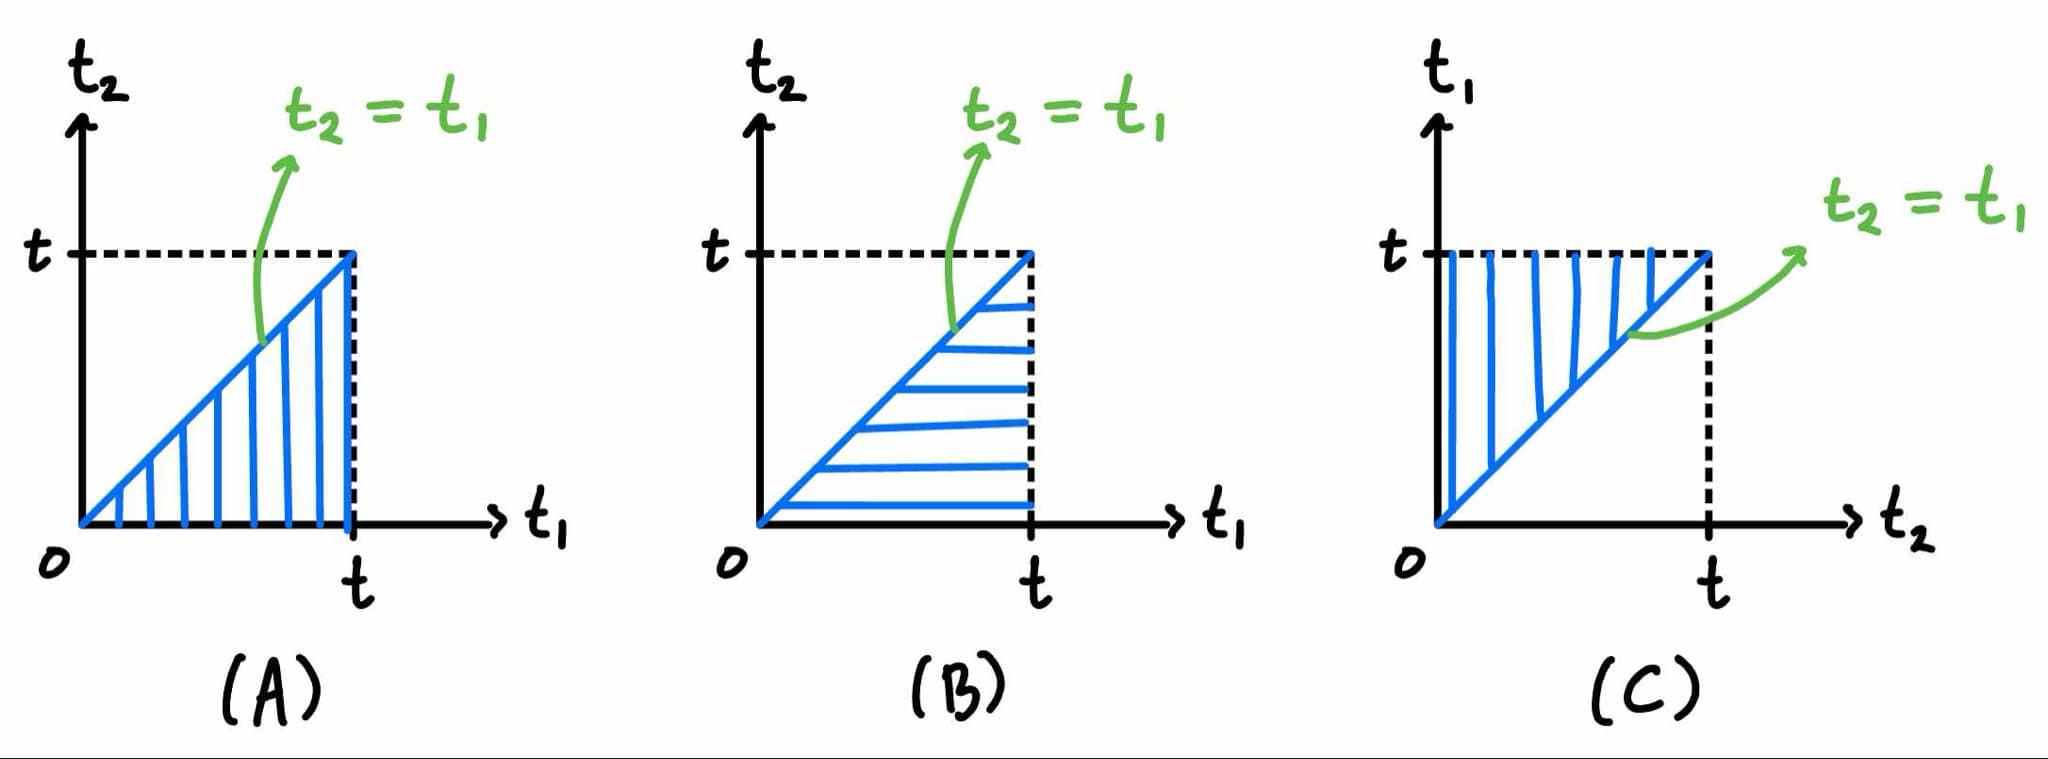
\includegraphics[width=0.6\textwidth]{images/ch1/region_integration.jpeg}
    \caption{Changements de la région d'intégration pour $J_2$}
\end{figure}


En général, pour $J_n$, il existera $n!$ façons différentes de l'écrire (pour les $n!$ façons d'organiser les $n$ hamiltoniens qui seront présents $\rightarrow$ les $n!$ changements de variables possibles). Par la suite, en sommant ces $n!$ équations, toutes les dépendances sur les $t_i$ partiront et la somme correspondra à $n!J_n$. Finalement, on isole $J_n$ pour obtenir 

\begin{equation}
    J_n = \frac{1}{n!}\int_{t_0}^{t}\int_{t_0}^{t}...\int_{t_0}^{t} T \left[H(t_1)H(t_2)...H(t_n)\right]dt_n ... dt_2 dt_1
\end{equation}

qu'on remplace dans (1.5) donnant ainsi

\begin{equation*}
    U(t,t_0) = \sum_{n=0}^{\infty}\frac{(-i)^n}{n!}\int_{t_0}^{t}\int_{t_0}^{t}...\int_{t_0}^{t} T \left[H(t_1)H(t_2)...H(t_n)\right]dt_n ... dt_2 dt_1
\end{equation*}

De là, si les hamiltoniens commutent (donc que $T$ ne fait rien), on voit qu'on peut retomber sur (1.4).

\begin{equation*}
    U(t,t_0) = \sum_{n=0}^{\infty}\frac{(-i)^n}{n!}\int_{t_0}^{t}\int_{t_0}^{t}...\int_{t_0}^{t}H(t_1)H(t_2)...H(t_n)dt_n ... dt_2 dt_1 = \sum_{n=0}^{\infty}\frac{(-i)^n}{n!}\left(\int_{t_0}^{t}H(t^{'})dt^{'}\right)^n
\end{equation*}
\begin{equation*}
    = \sum_{n=0}^{\infty}\frac{1}{n!}\left(-i\int_{t_0}^{t}H(t^{'})dt^{'}\right)^n = e^{-i\int_{t_0}^{t}H(t^{'})dt^{'}}
\end{equation*}

Dans les ouvrages, on utilise plutôt l'écriture

\begin{equation}
    U(t,t_0) = Te^{-i\int_{t_0}^{t}H(t^{'})dt^{'}} = \sum_{n=0}^{\infty}\frac{(-i)^n}{n!}\int_{t_0}^{t}\int_{t_0}^{t}...\int_{t_0}^{t} T \left[H(t_1)H(t_2)...H(t_n)\right]dt_n ... dt_2 dt_1
\end{equation}

\subsubsection{Écriture alternative}
Il peut être parfois plus logique d'écrire (1.5) selon l'ordre d'application des hamiltoniens sur un état (ce que certains auteurs préfèrent). On veut dire par là qu'on aimerait avoir l'indice $t_1$ pour l'hamiltonien le plus à droite, $t_2$ pour celui à sa gauche et $t_n$ pour l'hamiltonien le plus à gauche. Autrement dit, on veut renverser l'écriture de (1.5). On part depuis 

\begin{equation*}
    U(t,t_0) = \mathbb{I} -i\int_{t_0}^{t}H(t_1)U(t_1,t_0)dt_1
\end{equation*}

Auparavant, en remplaçant l'équation dans elle-même, on a 

\begin{equation*}
    U(t,t_0) = \mathbb{I} -i\int_{t_0}^{t}H(t_1)dt_1 - \int_{t_0}^{t}\int_{t_0}^{t_1}H(t_1)H(t_2)U(t_2,t_0)dt_2dt_1
\end{equation*}

Pour respecter la nouvelle notation, on a ici seulement besoin de renommer les variables du terme tout à droite.

\begin{equation*}
    U(t,t_0) = \mathbb{I} -i\int_{t_0}^{t}H(t_1)dt_1 - \int_{t_0}^{t}\int_{t_0}^{t_2}H(t_2)H(t_1)U(t_1,t_0)dt_1dt_2
\end{equation*}

En continuant le processus et en renommant les variables comme il faut, on obtient une forme générale pour cette notation alternative.

\begin{equation}
    U(t,t_0) = \sum_{n=0}^{\infty} (-i)^n \int_{t_0}^{t}\int_{t_0}^{t_n}...\int_{t_0}^{t_2}H(t_n)...H(t_1)dt_1 ... dt_{n-1} dt_n
\end{equation}


%ATTENTION AUX NUMÉROS D'ÉQ. FAIRE EN SORTE QUE ÇA SE SUIT.

% \subsection{Système ouvert}
% Pour l'instant, on s'est intéressé à l'équation de Schrödinger pour un système fermé, c'est-à-dire un système isolé de l'environnement. Cependant, un système quantique peut aussi intéragir avec son environnement et on qualifie le système comme étant ouvert. Dans ce cas, à la place d'un vecteur d'état (un ket), on a un ensemble statistique quantique (une distribution statistique d'états quantiques) qu'on représente par l'entremise d'une matrice densité $\rho(t)$.

% \begin{equation}
%     \rho(t) = \sum_{j}^{}p_j \ket{\psi_j(t)}\bra{\psi_j(t)} = \sum_{j}^{}p_j U(t,t_0)\ket{\psi_j(t_0)}\bra{\psi_j(t_0)}U^{\dagger}(t,t_0) = U(t,t_0)\rho(t_0)U^{\dagger}(t,t_0)
% \end{equation}

% Les $p_j$ correspondent aux probabilités de chaque état dans la distribution, donc $\sum_{j}^{}p_j = 1$ nécessairement. Par ailleurs, pour être physique, une matrice densité doit aussi être hermitienne ($\rho = \rho^{\dagger}$) et positive semi-définie ($\bra{\psi}\rho\ket{\psi} \geq 0$). Ces conditions assurent que les $p_j$ sont réels et $\geq 0$ (comme ça devrait être le cas pour des probabilités).

% En prenant la dérivée par rapport au temps de $\rho(t)$, on trouve 

% \begin{equation*}
%     \derivative{}{t}\rho(t) = \derivative{}{t}\left(U(t,t_0)\rho(t_0)U^{\dagger}(t,t_0)\right) = U(t,t_0)\rho(t_0)\left(\derivative{}{t}U^{\dagger}(t,t_0)\right) + \left(\derivative{}{t}U(t,t_0)\rho(t_0)\right)U^{\dagger}(t,t_0)
% \end{equation*}
% \begin{equation*}
%     = U(t,t_0)\rho(t_0)\left(\frac{\partial}{\partial t}U^{\dagger}(t,t_0)\right) + \left(\frac{\partial}{\partial t}U(t,t_0)\rho(t_0)\right)U^{\dagger}(t,t_0)
% \end{equation*}

% où, par (1.2), on peut déduire

% \begin{equation*}
%     \frac{\partial}{\partial t}U(t,t_0) = -iH(t)U(t,t_0) \implies \frac{\partial}{\partial t}U(t,t_0)\rho(t_0) = -iH(t)U(t,t_0)\rho(t_0)
% \end{equation*}
% \begin{equation*}
%     \frac{\partial}{\partial t}U^{\dagger}(t,t_0) = iU^{\dagger}(t,t_0)H^\dagger(t) 
% \end{equation*}

% de sorte que

% \begin{equation}
%     \derivative{}{t}\rho(t) = -i\left[H(t), \rho(t)\right]
% \end{equation}

% Cette dernière équation porte le nom d'équation de Liouville Von-Neumann.

% \subsection{Représentation d'Heisenberg}
% Depuis le début, l'objet mathématique qui effectue l'évolution temporelle est $U(t,t_0)$ et il s'applique sur un vecteur d'état/une matrice densité. En quelque sorte, on peut dire que "l'évolution est contenue" dans l'état/la matrice densité. Certes, les opérateurs peuvent dépendre ou non du temps, mais c'est bien l'état qui évolue. Cette façon d'écrire les choses se nomme la représentation de Schrödinger. 

% Tout de même, de manière équivalente, on pourrait "mettre l'évolution" dans les opérateurs, résultant en un état/une matrice densité qui ne dépendra plus du temps. C'est ce qu'on appelle la représentation de Heisenberg. Ainsi, il faut réussir à "transférer l'évolution" de l'état vers l'opérateur. Pour y arriver, on remarque que la valeur moyenne d'un opérateur $A(t)$ doit nécessairement être la même peu importe la représentation qu'on choisit.

% \begin{equation*}
%     \textlangle A(t)\textrangle = \text{Tr}(A(t)\rho(t)) = \text{Tr}(A_H(t)\rho(t_0)) 
% \end{equation*}

% Ici, $A(t)$ est la représentation de Schrödinger de l'opérateur (il ne contient pas l'évolution bien) tandis que $A_H(t)$ est sa représentation de Heisenberg (d'où le $H$ en dessous) contenant cette fois l'évolution. Sachant la définition de $\rho(t)$, on développe en utilisant une propriété de la trace :

% \begin{equation*}
%     \textlangle A(t)\textrangle = \text{Tr}(A(t)U(t,t_0)\rho(t_0)U^\dagger(t,t_0)) = \text{Tr}(A_H(t)\rho(t_0)) \implies \text{Tr}(U^\dagger(t,t_0)A(t)U(t,t_0)\rho(t_0)) = \text{Tr}(A_H(t)\rho(t_0)) 
% \end{equation*}
% \begin{equation}
%     \implies A_H(t) = U^\dagger(t,t_0)A(t)U(t,t_0)
% \end{equation}

% On sait maintenant grâce à (1.13) comment écrire l'évolution dans la représentation de Heisenberg. En dérivant (1.13) de chaque côté, on trouve 

% \begin{equation*}
%     \derivative{}{t}A_H(t) = \derivative{}{t}\left(U^\dagger(t,t_0)A(t)U(t,t_0)\right)
% \end{equation*}
% \begin{equation*}
%     = \left(\derivative{}{t}U^\dagger(t,t_0)\right)A(t)U(t,t_0) + U^\dagger(t,t_0)\left(\derivative{}{t}A(t)\right)U(t,t_0) + U^\dagger(t,t_0)A(t)\left(\derivative{}{t}U(t,t_0)\right)
% \end{equation*}
% \begin{equation*}
%     = \left(\frac{\partial}{\partial t}U^\dagger(t,t_0)\right)A(t)U(t,t_0) + U^\dagger(t,t_0)\left(\frac{\partial}{\partial t}A(t)\right)U(t,t_0) + U^\dagger(t,t_0)A(t)\left(\frac{\partial}{\partial t}U(t,t_0)\right)
% \end{equation*}
% \begin{equation*}
%     = iU^\dagger(t,t_0)H(t)A(t)U(t,t_0) + \underbrace{U^\dagger(t,t_0)\left(\frac{\partial}{\partial t}A(t)\right)U(t,t_0)}_\text{$\partial A_H(t)/\partial t$} - iU^\dagger(t,t_0)A(t)H(t)U(t,t_0)
% \end{equation*}

% Comme $\frac{\partial}{\partial t}A(t)$ et $H(t)$ sont aussi des opérateurs, (1.13) s'applique et on écrit

% \begin{equation*}
%     \derivative{}{t}A_H(t) = iU^\dagger(t,t_0)H(t)\underbrace{U(t,t_0)U^\dagger(t,t_0)}_\text{$\mathbb{I}$}A(t)U(t,t_0) - iU^\dagger(t,t_0)A(t)\underbrace{U(t,t_0)U^\dagger(t,t_0)}_\text{$\mathbb{I}$}H(t)U(t,t_0) + \frac{\partial}{\partial t}A_H(t)
% \end{equation*}
% \begin{equation}
%     = iH_H(t)A_H(t) -iA_H(t)H_H(t) + \frac{\partial}{\partial t}A_H(t) = i\left[H_H(t), A_H(t)\right] + \frac{\partial}{\partial t}A_H(t)
% \end{equation}

% où, juste pour clarifier la notation qui peut être mélangeante, 

% \begin{equation*}
%     \frac{\partial}{\partial t}A_H(t) = U^\dagger(t,t_0)\left(\frac{\partial}{\partial t}A(t)\right)U(t,t_0) 
% \end{equation*}

% À partir de (1.14), il est possible de calculer plusieurs cas limites ($H \text{ et/ou } A$ indé. temps, $A=H$, etc...). Avec ces équations, il est possible d'obtenir le fameux théorème d'Ehrenfest qui fait le lien entre la dérivée par rapport au temps de la valeur moyenne de $A$ dans chacune des représentations.

% \begin{equation*}
%     \derivative{}{t}\textlangle A(t)\textrangle = \derivative{}{t}\text{Tr}(A_H(t)\rho(t_0)) = \text{Tr}\left(\derivative{}{t}\left(A_H(t)\rho(t_0)\right)\right) = \text{Tr}\left(\left(\derivative{}{t}A_H(t)\right)\rho(t_0)\right) 
% \end{equation*}
% \begin{equation*}
%     = \text{Tr}\left(\left(i\left[H_H(t), A_H(t)\right] + \frac{\partial}{\partial t}A_H(t)\right)\rho(t_0)\right) = \text{Tr}\left(i\left[H_H(t), A_H(t)\right]\rho(t_0) + \frac{\partial}{\partial t}A_H(t)\rho(t_0)\right) 
% \end{equation*}
% \begin{equation}
%     = \text{Tr}\left(i\left[H_H(t), A_H(t)\right]\rho(t_0)\right) + \text{Tr}\left(\frac{\partial}{\partial t}A_H(t)\rho(t_0)\right) = \textlangle i\left[H_H(t), A_H(t)\right]\textrangle + \textlangle \frac{\partial}{\partial t}A_H(t)\textrangle
% \end{equation}


% \subsection{Représentation d'intéraction}
% Il existe une troisième représentation un peu plus générale que celles dont on vient de discuter. En effet, la représentation de Schrödinger et de Heisenberg sont deux cas spéciaux de ce qu'on appelle la représentation d'intéraction. Sans perte de généralité, on peut dire que tout hamiltonien s'écrit comme 

% \begin{equation*}
%     H(t) = H_0 + \hat{H}_{\text{int.}}(t)
% \end{equation*}

% où on sépare simplement la "partie constante" $H_0$ et la "partie dépendante du temps" $\hat{H}_{\text{int.}}(t)$ de l'hamiltonien $H(t)$. Dès lors, chaque hamiltonien présent, c'est-à-dire $H(t), H_0$ et $\hat{H}_{\text{int.}}(t)$, aura son propre opérateur d'évolution $U(t,t_0)$, $U_0(t,t_0)$ et $U_{\text{int.}}(t,t_0)$ respectivement. Comme $H_0$ ne dépend pas du temps, il va de soi par (1.3) que 

% \begin{equation*}
%     U_0(t,t_0) = e^{-iH_0(t-t_0)}
% \end{equation*}

% Pour clarifier, $H(t)$ est un hamiltonien qu'on aurait pu croiser avant cette section et donc $U(t,t_0)$ est de la même forme que (1.10). Pour $\hat{H}_{\text{int.}}(t,t_0)$, on peut tout bonnement dire que 

% \begin{equation*}
%     U_{\text{int.}}(t,t_0) = U^\dagger_0(t,t_0)U(t,t_0)
% \end{equation*}

% En effet, $U$ effectue l'évolution totale comprenant la partie constante et dépendante du temps. Si on évolue dans l'autre sens $U_0$ (d'où le $\dagger$), alors on annule seulement l'évolution de la partie constante. Ainsi, au final, la partie dépendante du temps est la seule à avoir évolué.

% Comme la valeur moyenne d'un opérateur ne change pas selon sa représentation, on trouve depuis la représentation de Schrödinger :

% \begin{equation*}
%     \textlangle A(t)\textrangle = \text{Tr}(A(t)\rho(t)) = \text{Tr}(A(t)U(t,t_0)\rho(t_0)U^\dagger(t,t_0))
% \end{equation*}
% \begin{equation*}
%     = \text{Tr}(\underbrace{U_0(t,t_0)U^\dagger_0(t,t_0)}_\text{$\mathbb{I}$}A(t)\underbrace{U_0(t,t_0)U^\dagger_0(t,t_0)}_\text{$\mathbb{I}$}U(t,t_0)\rho(t_0)U^\dagger(t,t_0))
% \end{equation*}
% \begin{equation*}
%     = \text{Tr}(U^\dagger_0(t,t_0)A(t)U_0(t,t_0)U^\dagger_0(t,t_0)U(t,t_0)\rho(t_0)U^\dagger(t,t_0)U_0(t,t_0))
% \end{equation*}
% \begin{equation}
%     = \text{Tr}(U^\dagger_0(t,t_0)A(t)U_0(t,t_0)U_{\text{int.}}(t,t_0)\rho(t_0)U^\dagger_{\text{int.}}(t,t_0)) = \text{Tr}\left(A_\text{int.}(t)\rho_\text{int.}(t)\right)
% \end{equation}

% où on pose 

% \begin{equation}
%     A_\text{int.}(t) = U^\dagger_0(t,t_0)A(t)U_0(t,t_0) 
% \end{equation}
% \begin{equation}
%     \rho_\text{int.}(t) = U_{\text{int.}}(t,t_0)\rho(t_0)U^\dagger_{\text{int.}}(t,t_0)
% \end{equation}

% Ces définitions ne tombent pas de nulle part, car elles permettent d'obtenir la représentation de Schrödinger ou de Heisenberg selon les conditions de chacune des représentations. Effectivement, si $\hat{H}_\text{int.}(t) = 0$, alors $H(t) = H_0 \implies U(t,t_0) = U_0(t,t_0)$ et $U_\text{int.}(t,t_0) = \mathbb{I}$. Dans ce cas, (1.16) devient

% \begin{equation*}
%     \textlangle A(t)\textrangle = \text{Tr}(U^\dagger_0(t,t_0)A(t)U_0(t,t_0)\rho(t_0)) = \text{Tr}(U^\dagger(t,t_0)A(t)U(t,t_0)\rho(t_0)) = \text{Tr}(A_H(t)\rho(t_0))   
% \end{equation*}

% ce qui correspond bien à ce qu'on devrait pour la représentation de Heisenberg. D'un autre côté, si $H_0 = 0$, un argument similaire permet de retomber sur la représentation de Schrödinger. Finalement, on peut adapter (1.2) et (1.12) pour prendre en compte la représentation d'intéraction.





